\section{Exact projection and a local game strategy}
\label{sec:projection}

Image consistency is necessary for equivalence by
Proposition~\ref{prop:image-consistency}. We now prove a converse for
twists concentrated in one row and at one end of each wire. This converse
requires only the individual image-set equalities: no simultaneous choice
of values from the sets is assumed.

Choose constants $b_e\in\F$, one for each comparison schema. For a link
$\ell$ on wire $e$, let $b_\ell=b_e$ if $\ell$ is the last link of the
wire and let $b_\ell=0$ otherwise. Set $\delta_r=1$ and $\delta_i=0$
for $1\leq i<r$. Define the square twist by
\begin{equation}
  \beta_B=\delta_i b_\ell
  \qquad\text{when $B$ is a square in row $i$ on link $\ell$.}
  \label{eq:special-twist}
\end{equation}
For this twist, the full-wire sum is $\Delta_e(a)=b_e$ at every
$a\in D_e$.

\begin{theorem}[Special-twist sufficiency]
\label{thm:special-twist}
Consider the graph construction with $r\geq32$ and $K=r+1$.
Let $\beta$ be given by Equation~\eqref{eq:special-twist}. Suppose that,
for every real type $P$ and every $a\in\{0,1\}^r$, there is a nonempty
set $Q_{P,a}\subseteq\F^{d_P}$, and that these sets satisfy
\begin{equation}
  \lambda_{e,0}(Q_{P,a})
  =b_e+\lambda_{e,1}(Q_{R,\sigma_e(a)})
  \qquad(e:P\longrightarrow R,\ a\in D_e).
  \label{eq:special-images}
\end{equation}
Then $G(0)\equiv_r G(\beta)$.
\end{theorem}

Throughout this section assume the hypotheses of the theorem. For each
internal type $s$ of wire $e:P\to R$, define
\begin{equation}
  Q_{s,a}:=\lambda_{e,0}(Q_{P,a})
       =b_e+\lambda_{e,1}(Q_{R,\sigma_e(a)})
       \qquad(a\in D_e).
  \label{eq:internal-image-set}
\end{equation}
These are nonempty scalar sets, independent of the internal type chosen
on that wire. We will assign offsets to the readouts of any collection
of at most $K$ blocks. Each assignment must translate legal homogeneous
valuations to legal shifted valuations. More strongly, every permitted
assignment on a smaller collection must extend to a permitted assignment
on a larger one. This extension property will let Duplicator preserve
old responses while preparing for every possible next vertex.

The sum around one address ring explains the form of these assignments.
Fix a type $t$ and an allowed address $a$, and put a vector $M_i$ at its
corner $(i,t,a_i)$, with $M_{r+1}=M_1$. If the horizontal offset in row $i$ is
$M_i+M_{i+1}+\delta_i h$, with $M_i,h\in\F^{d_t}$, then its sum around
the ring is $h$: every corner vector appears twice, while only row $r$
contributes $h$. We will call the corner vectors \emph{potentials}.
They allow the individual readouts to change while this sum stays fixed.
The proof will determine when the readouts constrain such a sum, and
when a change in the sum can be absorbed into the potentials.

\subsection{Small supports and wrapping addresses}

For a set $U$ of blocks, let $\Gamma_U$ be the undirected graph whose
edges are the readout names appearing in $U$, with their previously
defined corners as endpoints. Repeated names contribute only one edge.
A site contributes one horizontal edge; a square contributes its four
boundary edges. In particular, each block belongs to one connected
component of $\Gamma_U$. The \emph{type support} of a component is the
subgraph of the type layout consisting of its types and links.

\begin{lemma}
\label{lem:small-type-support}
If $|U|\leq K$, every component of $\Gamma_U$ has a type support that
is a tree with at most one real type. A support containing no real type
lies in a single wire interior. A support containing a real type consists
of that type and short arms in its incident wires.
\end{lemma}

\begin{proof}
The support is connected, because it is the image of a connected corner
graph. Each square contributes at most one distinct layout link, while
sites contribute none, so the support has at most $K$ links. Internal
types are private to their wires and have layout degree two. Consequently
a cycle, or a path between distinct real types, must traverse a complete
wire of $4K+1$ links. Neither fits into the support. The remaining
description follows by removing its possible real type.

The same argument allows loops and parallel comparison schemas. In
particular, two arms of one loop-wire may meet at its real endpoint, but
cannot meet again inside that wire without completing its long cycle.
\end{proof}

To compare labels at different types in such a support, fix, for every
link and boundary index, an extension of its label-matching injection to
a permutation of $\{0,1\}$. Use the identity for identity matches and
the inverse permutation when traversing a link backwards. Such
extensions exist because the coordinate maps are injections between
nonempty subsets of a two-element set. Choose a reference type in each
support tree. Transport along its unique paths then expresses all labels
at a given boundary index as labels at the reference type; call these
the \emph{aligned labels}. Every actual vertical edge preserves its
aligned label. On a connected subtree, the inherited alignment and the
alignment at a new reference differ only by re-expression at that
reference. This construction does not assert that every ambient label is
allowed at every internal type.

Give each horizontal edge in row $i$ the marker $\delta_i$, and each
vertical edge marker zero. A block collection, or a component of its
corner graph, is \emph{wrapping} if its corner graph has a closed walk
whose marker sum in $\F$ is one. Thus wrapping means that some closed
walk crosses the row-$r$ seam an odd number of times. Traversals in either
direction have the same marker.

\begin{lemma}[Wrapping addresses]
\label{lem:wrapping-address}
Let $|U|\leq r+1$.
\begin{enumerate}
\item Every wrapping subcollection of $U$ has at least $r$ blocks.
\item A wrapping collection of exactly $r$ blocks has one block in
each row, lies in one component, and determines a full address in that
component's aligned labels.
\item All wrapping $r$-subcollections of $U$, if any, lie in one
component of $\Gamma_U$ and determine the same aligned address there.
\end{enumerate}
\end{lemma}

\begin{proof}
For a closed walk, let $c_i\in\F$ be its horizontal traversal count
in row $i$, reduced modulo two. Summing incidences at all corners with
boundary index $i$ gives $c_{i-1}=c_i$: vertical traversals contribute
twice. An odd marker means $c_r=1$, so every row has an odd horizontal
traversal count. Since a block supplies horizontal edges in only its own
row, at least $r$ blocks are needed.

If there are exactly $r$ blocks, there is one in each row, and the walk
meets every block. Thus all blocks lie in its component. The horizontal
edge of a site, or the two horizontal edges of a square, prescribes one
pair of aligned labels for that row. In the square case the two edges
give the same pair because vertical edges preserve alignment. Now sum
the walk's incidences separately at each aligned label of boundary
index $i$. Vertical contributions again cancel. The odd horizontal
traversal counts in the adjacent rows force their prescribed labels at
this boundary to agree. Doing this at every boundary gives the full
address.

Two $r$-subcollections of $U$ share at least $r-1$ blocks. For wrapping
subcollections these common blocks belong to distinct rows and put both
subcollections in the same component. The common rows, all but at most
one row, touch every boundary index because $r\geq3$. Hence they force
the two addresses to agree at every coordinate.
\end{proof}

\subsection{Translations on a small block collection}

We next define the translations that will be available to Duplicator.
The address condition will be imposed only when a wrapping collection
of exactly $r$ blocks is present. A wrapping component with $r+1$
blocks need not contain such a collection; this distinction is essential
when restricting to smaller collections.

Fix $U$ with $|U|\leq K$. In each component $C$ of $\Gamma_U$, choose
a vector $h_t\in\F^{d_t}$ for each type in its support, subject to
\begin{equation}
  L_{\ell,t}(h_t)+L_{\ell,u}(h_u)=b_\ell
  \qquad(\ell=tu\text{ in the support}).
  \label{eq:component-shifts}
\end{equation}
The choices are made separately in distinct corner components, even
when the same type occurs in more than one component. If $C$ contains
a wrapping $r$-subcollection, use its unique aligned address from
Lemma~\ref{lem:wrapping-address} and impose one further condition:
\begin{itemize}
\item If the support contains a real type $P$, require
$h_P\in Q_{P,a}$, where $a$ is the address expressed at $P$.
\item If the support has no real type, require its common internal
scalar to lie in $Q_{s,a}$, where $a$ is expressed in the source
coordinates of its wire.
\end{itemize}
In the second case, $a\in D_e$: every boundary label of the wrapping
collection is read at an internal type of wire $e$, and its interior
matches are identities. In the first case every address is permitted
at $P$; there is no additional address-dependent condition on its arms.
If no wrapping $r$-subcollection is present, impose only
Equation~\eqref{eq:component-shifts}. Call shifts satisfying these
requirements \emph{admissible}.

Admissible shifts always exist. In a wire interior all $b_\ell$ vanish,
so one common scalar, in the indicated nonempty set when required,
suffices. If the support contains a real type, choose its vector
arbitrarily or from the indicated nonempty $Q$ set. Its endpoint forms
then determine the scalar on each arm, adding the last-link constant
when that arm meets the second endpoint of a wire. The scalar is
constant along the rest of the arm. Distinct arms have private internal
types, so these choices do not conflict, even when an endpoint form
vanishes.

Independently choose a potential $M_v\in\F^{d_t}$ at every corner $v$
of type $t$. Define offsets on the readouts by
\begin{equation}
\begin{aligned}
  x_{vw}&=M_v+M_w+\delta_i h_t
    &&\text{for a horizontal edge in row $i$ at type $t$},\\
  y_{vw}&=L_{\ell,t}(M_v)+L_{\ell,u}(M_w)
    &&\text{for a vertical edge on $\ell=tu$}.
\end{aligned}
\label{eq:potential-offsets}
\end{equation}
The endpoints of the vertical edge are ordered as in its readout name.
Let $\mathcal H_U$ be the family of all assignments to the readout names
of $U$ obtained this way. Set $\mathcal H_\varnothing=\{\varnothing\}$.
Every family is nonempty. In a square, the potential terms cancel and
the remaining offset sum is
\[
  \delta_i\bigl(L_{\ell,t}(h_t)+L_{\ell,u}(h_u)\bigr)
  =\delta_i b_\ell=\beta_B.
\]
Thus every assignment in $\mathcal H_U$ satisfies
Equation~\eqref{eq:square} on all squares in $U$. It translates every
homogeneous block valuation into a legal valuation for the twist.
Shared readouts receive the same offsets because they are the same
edges of $\Gamma_U$. Figure~\ref{fig:projection-gauge} shows how the
potentials preserve old readouts when a site ring is cut. The next proof
extends this adjustment to every nonwrapping component.

\begin{figure}[htbp]
\centering
\begin{minipage}[t]{0.47\linewidth}
\centering
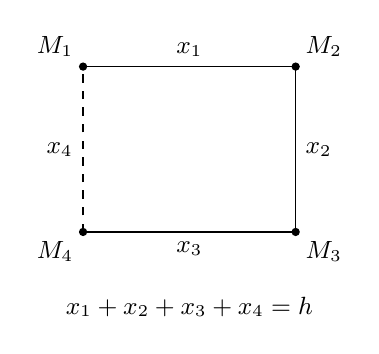
\begin{tikzpicture}[font=\small,line width=0.5pt]
 \coordinate (v1) at (0,0);
 \coordinate (v2) at (2.7,0);
 \coordinate (v3) at (2.7,-2.1);
 \coordinate (v4) at (0,-2.1);
 \draw (v1)--node[above]{$x_1$}(v2)
       --node[right]{$x_2$}(v3)
       --node[below]{$x_3$}(v4);
 \draw[dashed,thick] (v4)--node[left]{$x_4$}(v1);
 \foreach \v in {v1,v2,v3,v4} \fill (\v) circle (1.5pt);
 \node[above left] at (v1) {$M_1$};
 \node[above right] at (v2) {$M_2$};
 \node[below right] at (v3) {$M_3$};
 \node[below left] at (v4) {$M_4$};
 \node at (1.35,-3.05) {$x_1+x_2+x_3+x_4=h$};
\end{tikzpicture}
\end{minipage}\hfill
\begin{minipage}[t]{0.50\linewidth}
\centering
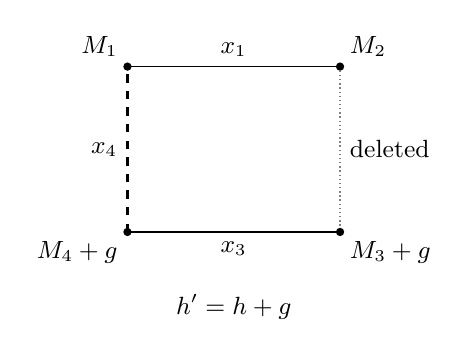
\begin{tikzpicture}[font=\small,line width=0.5pt]
 \coordinate (v1) at (0,0);
 \coordinate (v2) at (2.7,0);
 \coordinate (v3) at (2.7,-2.1);
 \coordinate (v4) at (0,-2.1);
 \draw (v1)--node[above]{$x_1$}(v2);
 \draw[densely dotted,gray] (v2)--node[right,text=black]{deleted}(v3);
 \draw (v3)--node[below]{$x_3$}(v4);
 \draw[dashed,thick] (v4)--node[left]{$x_4$}(v1);
 \foreach \v in {v1,v2,v3,v4} \fill (\v) circle (1.5pt);
 \node[above left] at (v1) {$M_1$};
 \node[above right] at (v2) {$M_2$};
 \node[below right] at (v3) {$M_3+g$};
 \node[below left] at (v4) {$M_4+g$};
 \node[align=center] at (1.35,-3.05)
   {$h'=h+g$};
\end{tikzpicture}
\end{minipage}
\caption{A schematic site ring at one type and one address, drawn with four
rows; the construction itself uses $r\ge32$. Here $x_i$ is the horizontal
offset in row $i$, and $g$ is any vector in the same space as $h$.
The dashed edge is the row-$4$ seam. Left: every potential occurs twice in the sum, leaving $h$.
Right: after deleting row $2$, changing $h$ to $h+g$ and adding $g$ to
$M_3,M_4$ preserves every retained readout. The dotted segment is absent
from the retained corner graph. The proof of
Proposition~\ref{prop:exact-projection} makes this adjustment on each
nonwrapping old component, including components meeting several types. Adapted from \cite[Figure~2]{VariableWL}.}
\label{fig:projection-gauge}
\end{figure}

\subsection{Exact projection}

The families just constructed provide legal translations on small
collections. Their usefulness in the game depends on preserving every
old readout when the block collection grows.

A proper old collection has at most $r$ blocks. If an old component
wraps, it uses all $r$ of them and carries the only old choice subject to
an address-set condition. We will retain its chosen shifts, or lift its
scalar through an endpoint form. On every other old component,
the marker can be expressed as a sum of binary values at the edge
endpoints. There we can change the component shifts and compensate by
changing potentials, leaving all old
readouts unchanged. These are the two cases of the following proof.

\begin{proposition}[Exact projection]
\label{prop:exact-projection}
For $V\subseteq U$ with $|U|\leq r+1$, restriction to the readout names
occurring in $V$ maps $\mathcal H_U$ onto $\mathcal H_V$.
\end{proposition}

\begin{proof}
The assertion is immediate for $V=U$. Assume $V\subsetneq U$, so
$|V|\leq r$. Each component $D$ of $\Gamma_V$ lies in a component
$C$ of $\Gamma_U$, and its type support is a subtree of that of $C$.

\emph{Restriction of admissible shifts.}
If $D$ is nonwrapping,
it has no $Q$ requirement, so restriction causes no problem. If $D$
wraps, its blocks form a wrapping $r$-collection by
Lemma~\ref{lem:wrapping-address}; in particular they exhaust $V$.
The address imposed on $C$ restricts to the same address on $D$.
When $D$ contains a real type, it is the same real type as in $C$ and
has the same $Q$ requirement. When $C$ has no real type, both supports
are in one wire interior and require the same common scalar.

The remaining case is that $D$ lies inside a wire and $C$ reaches one
of its real endpoints. The address $a$ read inside $D$ belongs to the
actual product domain $D_e$. Consequently its expression at the real
endpoint uses actual endpoint matches: it is $a$ at the first endpoint
and $\sigma_e(a)$ at the second. By
Equation~\eqref{eq:internal-image-set}, the permitted internal scalar
set is exactly the image of the permitted real-vector set under the
endpoint form, translated by the end-link constant if present.
Restriction is therefore admissible. The same equality shows that any
permitted internal scalar has a permitted real-vector preimage.

\emph{Extension from a wrapping old component.}
These cases also show that admissible shifts on a wrapping old component
extend to admissible shifts on its containing new component: retain its
real vector if already present, retain its scalar if the new support
remains internal, or choose the real preimage just described. Then
extend along the remaining arms. Only one arm is constrained in the
preimage case. Since a wrapping old component consumes all $r$ old
blocks, there is never a second old wrapping choice to lift
simultaneously. This remains true for loop-wires whose two original
endpoints are the same real type.

\emph{Preservation of every old readout.}
Restricting the potentials as well now proves that every restriction of
an element of $\mathcal H_U$ lies in $\mathcal H_V$. For surjectivity,
fix a representation of an element of $\mathcal H_V$ by old shifts and
potentials. Choose admissible shifts on $U$, agreeing with the old
shifts on the possible wrapping old component; the preceding argument
shows this is possible. We will adjust potentials to preserve the old
readouts on every nonwrapping component $D$.

On such a component, the marker is a difference of corner labels:
there are $s_v\in\F$ with marker $s_v+s_w$ on each edge $vw$.
Indeed, choose path sums from one fixed corner. They are well-defined
because every closed walk has marker sum zero. Let $g_t$ be the sum of
the new and old shifts at type $t$ in this component. Their identical
inhomogeneous link equations imply
\[
  L_{\ell,t}(g_t)+L_{\ell,u}(g_u)=0
  \qquad(\ell=tu\text{ in the support of }D).
\]
Replace the old potential at $v$ of type $t$ by $M_v+s_vg_t$.
For a horizontal edge in row $i$, the resulting change in its offset,
including the change of shift, is
\[
  (s_v+s_w+\delta_i)g_t=0.
\]
For a vertical edge, $s_v=s_w$, and the homogeneous link equation makes
its offset change zero as well. Hence every old readout is preserved.

Different old components have disjoint corners, so their potential
adjustments are compatible even if they merge in $\Gamma_U$ or contain
the same type. Retain the old potentials on a wrapping old component
and choose arbitrary potentials at all new corners. Together these
choices give an element of $\mathcal H_U$ extending the prescribed
element of $\mathcal H_V$.
\end{proof}

In particular, a wrapping $(r+1)$-block component with no wrapping
$r$-subcollection causes no exceptional case. Every proper subcollection
has at most $r$ blocks and is nonwrapping, so the potential adjustment
in the proof applies without a $Q$ restriction.

\subsection{From translations to a vertex bijection}

We can now prove Theorem~\ref{thm:special-twist}. Fix the following
ownership convention, identically in $G(0)$ and $G(\beta)$. A block's
valuation vertices are owned by that block. Each bit-value pair is
owned by one fixed block using its readout name. Such a block exists:
horizontal names have sites, and every vertical name belongs to a
square because the adjacent coordinate domains are nonempty. A leaf
has its parent's owner and a fixed private index among the leaves at
that parent.

\begin{proof}[Proof of Theorem~\ref{thm:special-twist}]
Duplicator maintains an assignment in $\mathcal H_U$, where $U$ is
the set of owners of the currently marked vertices. Marked base
vertices are matched by translation using the offsets on their
owners: translate each block valuation and each bit-value coordinate.
A marked leaf is sent to the leaf with the same private index at the
translated parent. Since $|U|$ is at most the number of occupied slots,
the family $\mathcal H_U$ is always defined.

For any fixed assignment, translation is bijective on every base
vertex class with owner in $U$: it maps homogeneous legal valuations
onto the legal valuations for the twist, and permutes each bit-value
pair. Parent translation also gives a bijection on the corresponding
leaves, since translated parents have the same color and hence the
same number of attached leaves.

These translations give a partial isomorphism on the marked vertices.
The only possible base incidence is between a block valuation and a
bit-value vertex for a coordinate used by that block. When both are
marked, their owners belong to $U$ and the common readout receives
one offset. Equality or inequality of the two bits is therefore
preserved, so both adjacency and nonadjacency are preserved. All other
pairs of base classes have no edges in either graph. Leaf attachments
are preserved by parent translation and private indices. Translation
within each class is injective, distinct classes remain distinct, and
leaf indices are preserved, so equality of marked vertices is
preserved as well.

Discarding pairs simply restricts the maintained assignment to the
remaining owners, which is allowed by
Proposition~\ref{prop:exact-projection}. Suppose now that a slot is
vacant. There are at most $K-1=r$ current owners. For \emph{each}
possible owner $B$ of the next vertex, choose an extension of the
current assignment to $\mathcal H_{U\cup\{B\}}$. This is possible
before any vertex is selected, by exact projection. If $B\in U$, use
the current assignment itself.

On the part of the vertex set owned by $B$, use the chosen extension
to translate the base classes and their leaves. These parts partition
the vertex set, and each maps bijectively onto the identically owned
part in the other graph. They therefore combine into a single vertex
bijection, which Duplicator announces. Its parts for the current
owners agree with the maintained assignment, so in particular it
extends all currently marked pairs, including repeated occurrences of
a vertex.

After Spoiler selects a vertex, retain the extension chosen for its
owner $B$. It agrees with every old marked pair and with the newly
selected pair. The preceding partial-isomorphism check applies to
this enlarged position. Thus the strategy wins with $K=r+1$ slots,
which proves $G(0)\equiv_r G(\beta)$.
\end{proof}
